\documentclass[12pt, twoside, a4paper, DIV12, BCOR16mm]{scrartcl}
%scrartcl und fancyhdr sind nicht kompatibel
\makeatletter
\DeclareOldFontCommand{\rm}{\normalfont\rmfamily}{\mathrm}
\DeclareOldFontCommand{\sf}{\normalfont\sffamily}{\mathsf}
\DeclareOldFontCommand{\tt}{\normalfont\ttfamily}{\mathtt}
\DeclareOldFontCommand{\bf}{\normalfont\bfseries}{\mathbf}
\DeclareOldFontCommand{\it}{\normalfont\itshape}{\mathit}
\DeclareOldFontCommand{\sl}{\normalfont\slshape}{\@nomath\sl}
\DeclareOldFontCommand{\sc}{\normalfont\scshape}{\@nomath\sc}
\makeatother

%Ländereinstellungen
\usepackage[english, german]{babel}

%Grafiken, erweiterte Kopf- und Fußzeilen, Seienreferenzvariablen, Listings, erweiterte Symbole,
%deutsche Literatur Formatierung, zeilen-übergreifende Kommentare, Textmarkierungen
\usepackage{graphicx, fancyhdr, lastpage, listings, wasysym,
	bibgerm, comment, changebar, subfigure}
\usepackage[usenames, dvipsnames]{color} %für mehr Farben
% weiter evtl. nützliche Packages: ifthen, wasysym, changebar, supertabular

\usepackage[onehalfspacing]{setspace}

%\usepackage{palatino}% weitere Schriftarten

\usepackage[utf8]{inputenc} % Umlaute richtig verarbeiten  
\usepackage[T1]{fontenc}      % Feinheiten im Satz von Umlauten



% Packages, die 'bessere' PDF-Dokumente erzeugen 
\usepackage{ae} 
\usepackage[
pdftitle={Ausarbeitung}
bookmarks=true,
bookmarksnumbered=true, % Verwendete Bookmarks anzeigen
colorlinks,   % Farbige Links
linkcolor=black,
urlcolor=blue,
citecolor=black]{hyperref}
%\usepackage[dvips]{thumbpdf}

% Legt die Einrücktiefe der ersten Zeile für aller Absätze fest. (0:=Absätze nicht einrücken)
\setlength{\parindent}{0pt}  
%\parskip1ex plus0.5ex minus0.5ex   

% Legt die Breite des Randnotizen-Bereichs festlegen (auch über BCORxxx konfigurierbar)
%\setlength{\marginparwidth}{25mm}
%\evensidemargin0mm
%\oddsidemargin8mm

% Definiert die Gesamthöhe des Textrumpfes für alle nachfolgenden Seiten.
\setlength{\textheight}{225mm}
\setlength{\headheight}{13mm}
\setlength{\topskip}{10mm}

% Nummerierungstiefe des Inhaltsverzeichnis 
\setcounter{tocdepth}{3} % auch {3} ist OK aber bitte nicht mehr

% Kopfzeilenformatierung
%\fancyhead[RO,LE]{\small \sffamily Inhalt} 
%\fancyhead[LO,RE]{\small \sffamily Beispiel für ein \LaTeX\ Dokument} 



\begin{document}
 \addsec{Datenanalyse}
\addsec{Perzeptron}
Das Perzeptron ist eine Form von künstlichen neuronalen Netzen. Dabei wird zwischen einlagigen und mehrlagigen Perzeptrons unterschieden.  Das Perzeptron wandelt einen Eingabevektor zu einem Ausgabevektor um. Bei einem einlagigen Perzeptron ist der Eingabevektor gleich der Ausgabevektor. Es lassen sich damit nur linear separable Mengen trennen. Nur die AND-Funktion ist linear separabel, die XOR-Funktion ist dagegen nicht linear separabel. 
\begin{figure}[h]
	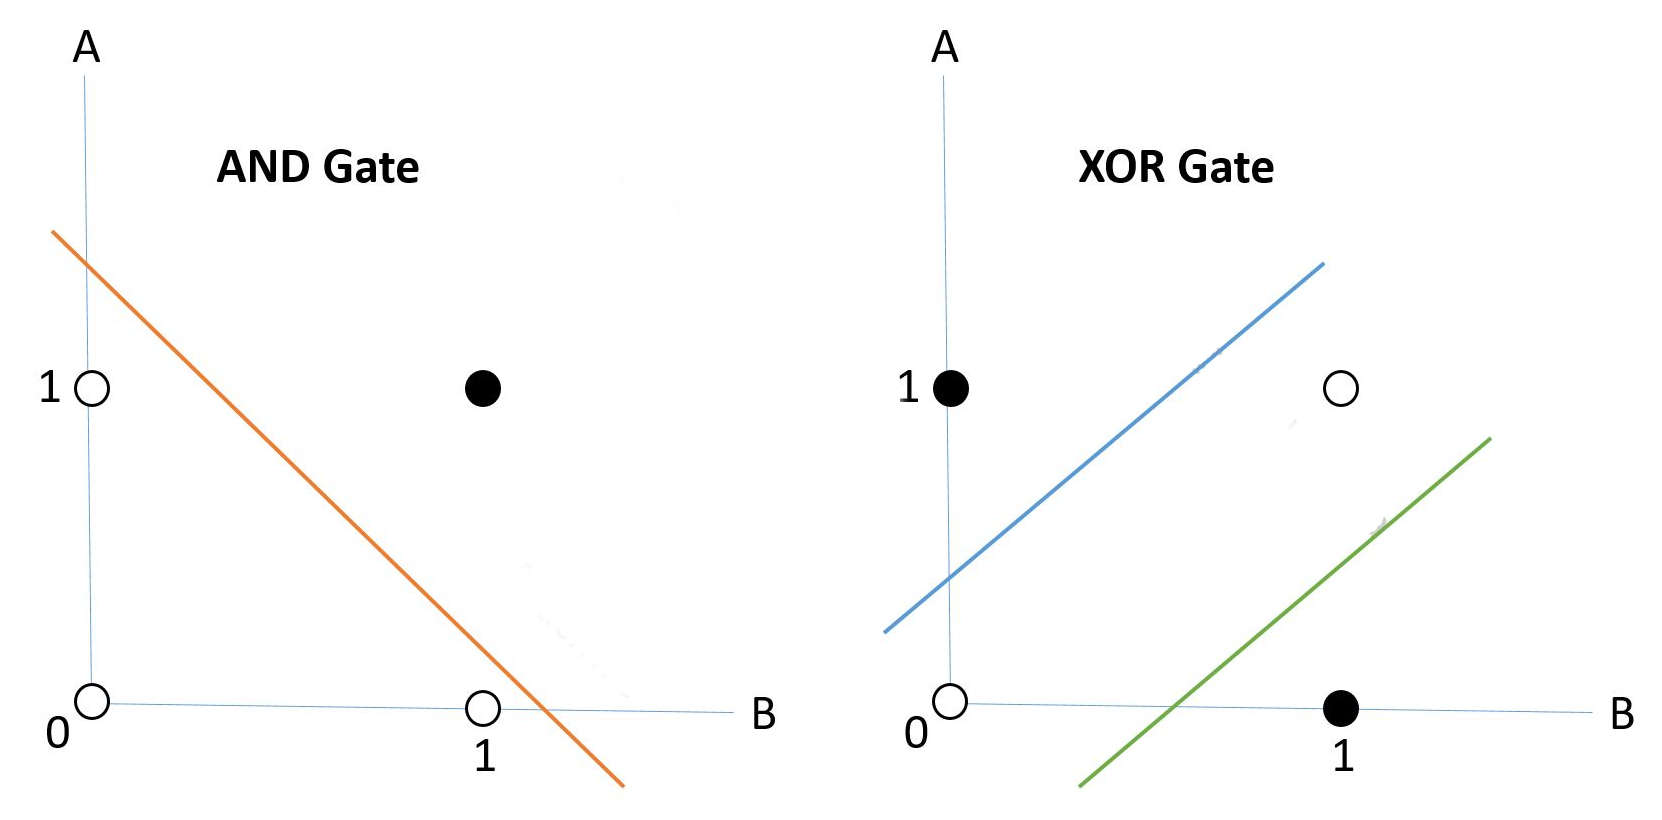
\includegraphics[width=1\linewidth]{Bilder/perzeptron_and_xor}
	\caption{AND ist linear separabel, XOR hingegen nicht}\label{Perzeptron}
\end{figure}
\\
Das Perzeptron kann jedoch nicht beliebige linear separable Mengen trennen, sondern nur welche durch eine Ursprungsgerade oder durch eine Hyperebene im Ursprung trennbar sind.
\\
 Zuerst muss das Perzeptron mit Trainingsdaten trainiert werden, damit sich neue Eingabevektoren klassifizieren lassen. Dabei wird im ersten Schritt ein zufälliger Gewischtverktor initialisiert. Im nächsten Schritt werden alle Mengen geprüft ob sie richtig eingeordnet wurden, ist dies nicht der Fall, werden Gewichte addiert oder subtrahiert bis die Gerade konvergiert und alle Mengen richtig klassifiziert sind. Tritt keine konvergenz ein, sind die beiden Mengen nicht linear separabel. Die Konvergenz Zeit der Geraden hängt stark vom initial Gewichtsvektor ab. Im besten Fall Konvergiert die Gerade direkt beim ersten Durchlauf. Durch heuristische verfahren kann eine möglichste beste Initialisierung erreicht werden um eine schnelle Konvergenz zu erreichen. 
\\\\
Das mehrlagige Perzeptron ist in der Lage auch nicht linear separable Mengen zu trennen. Neben der Eingabe- und Ausgabeschicht gibt es dazwischen noch sogenannte hidden layer.
\begin{figure}[h]
	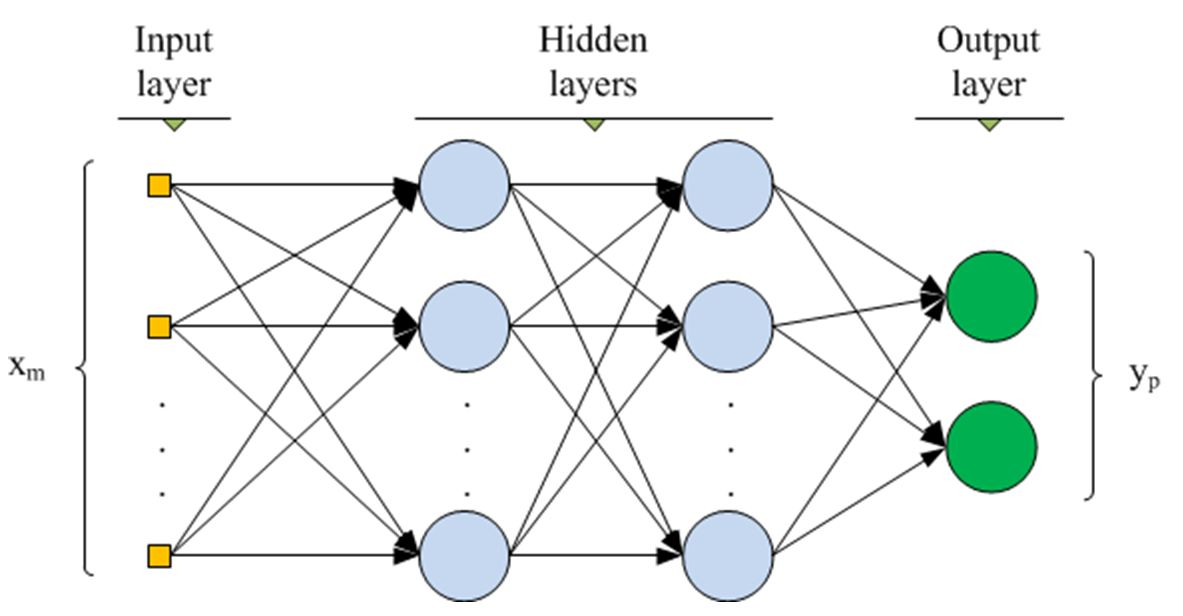
\includegraphics[width=1\linewidth]{Bilder/multilayer_perzeptron}
	\caption{Mehrlagiges Perzeptron}\label{Perzeptron}
\end{figure} 
Dabei sind immer alle Neuronen einer Schicht mit der nächsten Schicht verbunden. Dieses kann mit dem Backpropagnation Algorithmus trainiert werden. Beim Erlernen sollen möglichst genaue Abbildungen der Eingabevektoren auf die Ausgabevektoren entstehen. Die Genauigkeit wird durch eine Fehlerfunktion beschrieben.  Im ersten Schritt wird der Eingabevektor vorwärts durch das Netz propagiert. Anschließend wird die Fehlerrate vom Ausgabevektor zum Eingabevektor berechnet.  Diese wird nun beim Rückwärtspropaginieren verwendet und von Schicht zu Schicht die Gewichte angepasst. Dies wird solange wiederholt bis sich die Gewichte nicht mehr ändern. 

\addsec{Nearest neighbour}

Im Gegensatz zum Perzeptron gehen beim Nearest Neighbour Algorithmus keine Informationen über die Daten verloren. Da beim Perzeptron das vorhandene Wissen der Trainingsdaten in den Gewichtsvektor umgewandelt wird. Das ist aber unerwünscht, da die Trainingsdaten generalisiert werden sollen um eine Funktion zu finden, die die Daten möglichst genau klassifiziert. Beim Nearest Neighbour wird der Abstand zum nächsten Punkt gemessen und der jeweiligen Klasse zugeordnet.
\\\\
 Hat ein Punkt mehrere Merkmale ist es sinnvoll den jeweiligen Merkmalen Gewichte zuzuordnen um eine bessere Klassifizierung zu ermöglichen. Im Gegensatz zum Perzetron müssen die Mengen nicht linear separabel sein. Wird jedoch ein Punkt falsch klassifiziert, kann es sein, dass darauffolgende Punkte auch falsch klassifiziert werden, da sie den geringsten Abstand vorweisen. Um dies zu verhindern kann die K-Nearest Neighbour Methode angewendet werden, hier wird nicht der nächste Nachbar ermittelt, sondern die k-nächsten Nachbarn.
 \begin{figure}[h]
 	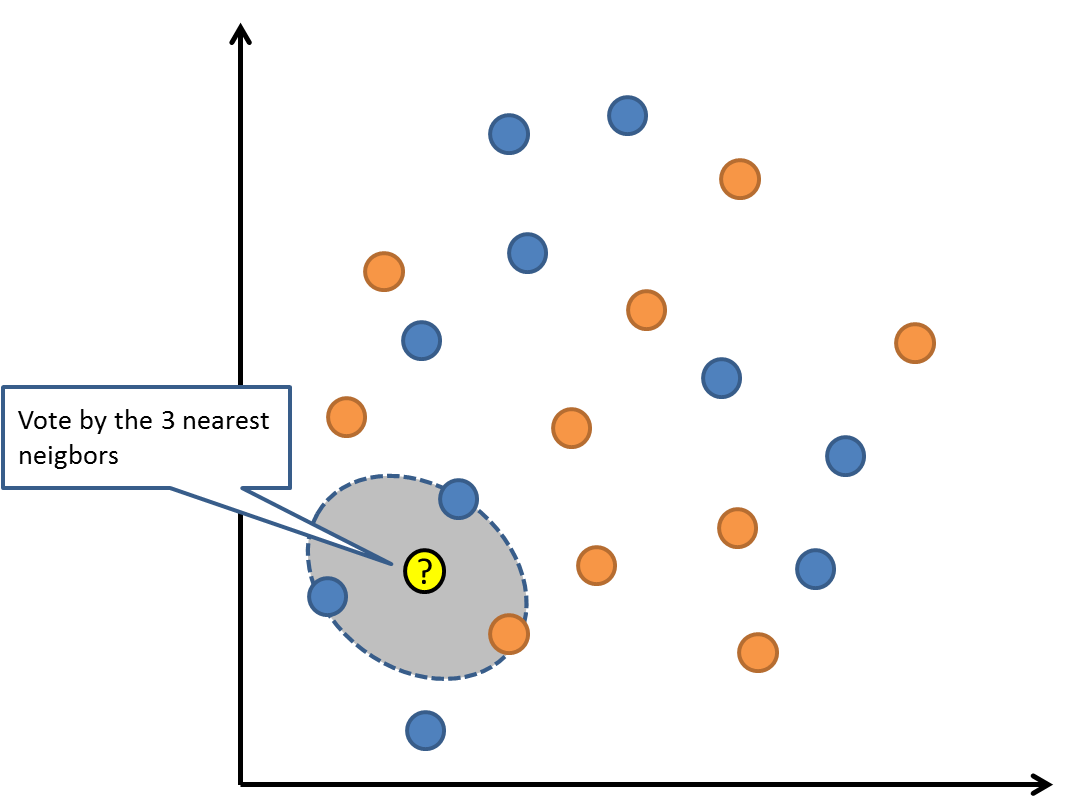
\includegraphics[width=1\linewidth]{Bilder/k_nearest_neighbour}
 	\caption{k-Nearest Neighbour mit k=3}\label{nearest_neigbour}
 \end{figure}  \\
Dadurch ist die Gefahr einer falsch Klassifizierung geringer und eine Überanpassung wird verhindert. Ein weiterer Vorteil der Nearest Neighbour Methode im Gegensatz zum Perzeptron ist, dass es auch mehr als zwei Klassen geben kann. Bei wachsendem K gibt es viele Nachbarn die einen großen Abstand zum klassifizierendem Punkt aufweisen. Daher müssen die Nachbarn gewichtet werden, damit näher liegende Nachbarn einen größeren Einfluss auf die Klassifizierung nehmen. Dazu können verschiedene Formeln verwendet werden um den Abstand der Nachbarn zu berechnen. Der Rechenaufwand der nächsten Nachbarn wächst linear mit der Anzahl der Daten. Dies kann bei einer sehr großen Anzahl an Daten zu einem Problem werden.
\\
\newline
Beim Perzeptron handelt es sich um ein Eager Learning (eifriges Lernen) Algorithmus, hierbei ist das Lernen sehr aufwändig, jedoch können neue Datenpunkt anschließend ganz einfach klassifiziert werden, indem sie in den Gewichstverktor eingesetzt werden. Beim Nearest Neighbour handelt es sich um ein Lazy Learning (faules Lernen) Algorithmus, dabei ist kein Lernen erforderlich, jedoch dauert die anschließende Klassifizierung neuer Datenpunkte deutlich länger, da zu jedem Punkt der Abstand berechnet werden muss.

\newpage
\addsec{Clustering}
Beim Clustering werden Daten mit Ähnlichkeiten zu Gruppen zusammengefasst, diese werden als Cluster bezeichnet. Der Unterschied zu den anderen Algorithmen ist, dass es sich hierbei um ein Lernen ohne Lehrer handelt. Denn die Trainingsdaten müssen nicht klassifiziert sein. Hier sollen Häufigkeiten der Daten erkannt werden und zu Clustern zusammengefasst werden. Die Abstände der Daten sind in einem Cluster geringer als der Abstand zu den nächsten Clustern, da die Daten eine Ähnlichkeit aufweisen.
 \begin{figure}[h]
	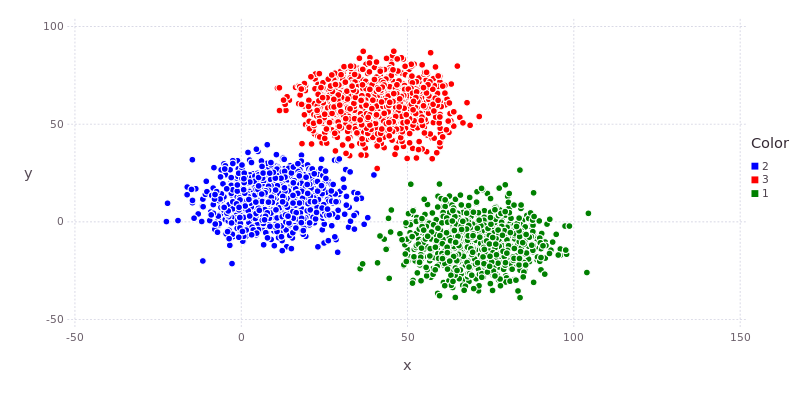
\includegraphics[width=1\linewidth]{Bilder/clustering}
	\caption{Clustering}\label{clustering}
\end{figure}  

\addsec{Partitionierende Clusterverfahren}
Bei sogenannten partitionierenden Clusterverfahren muss die Anzahl der Cluster k bekannt sein. Dann werden k Clusterzentren initialisiert und so lange verschoben bis sich keine Änderungen der Cluster ergeben. 
\newline
\textbf{K-Means-Algorithmus}\\
Dazu müssen am Anfang die Anzahl der Cluster k bekannt gegeben werden. Anschließend die k-Clusterzentren zufällig initialisiert und der Abstand zu den nächsten Daten berechnet und dementsprechend den Clustern zugeordnet. Nun wird das neue Mittelwert des Clusters berechnet und der vorherige Schritt widerholt bis es keine Änderungen der Clusterzentren mehr gibt. Das Problem dabei ist, dass die Anzahl der Cluster bereits zu Beginn bekannt sein müssen. Häufig ist dies jedoch nicht der Fall.
\newline
\textbf{EM-Algorithmus}\\
Der Expectation-Maximization-Algorithmus ist in zwei Schritte aufgeteilt, in Expectation und Maximization. Dabei wird beim Expectation Schritt für jeden Datenpunkt die Wahrscheinlichkeit berechnet, zu welchem Cluster er gehört. Anschließend wird im Maximization Schritt die Parameterverteilung neu berechnet unter Verwendung der errechneten Wahrscheinlichkeitsverteilung vom vorherigen Schritt. Dadurch ist meinst eine bessere Einteilung der Cluster möglich.
\addsec{Hierarchisches Clustering}
Der Vorteil hierbei ist, dass die Anzahl der Cluster zu Beginn nicht bekannt sein müssen. Im ersten Schritt werden mit n Clustern gestartet. Dabei stellt jeder Datenpunkt ein Cluster dar.
 \begin{figure}[h]
	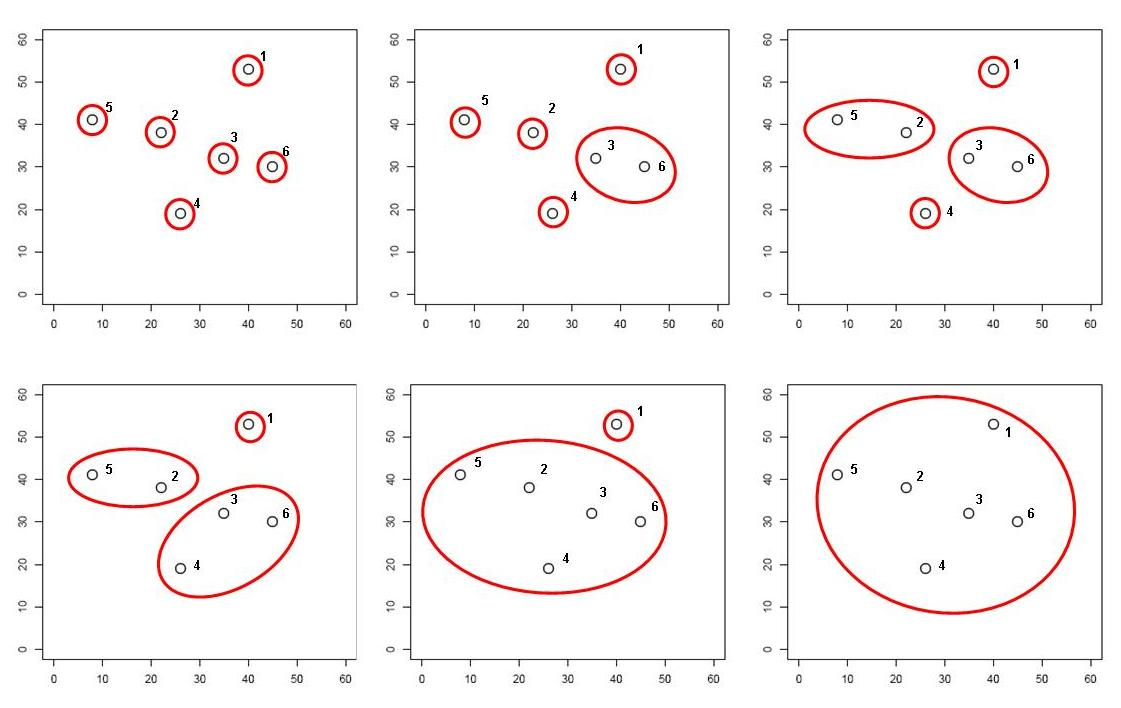
\includegraphics[width=1\linewidth]{Bilder/hierarchisches_clustering}
	\caption{Hierarchisches Clustering}\label{hierarchisches_clustering}
\end{figure}  
 Anschließend werden jeweils die nächsten Nachbarcluster vereinigt, bis ein Abbruchkriterium erreicht wird oder alle Datenpunkte zu einem Cluster zusammengefasst sind. Ein Grund für einen Abbruch kann ein maximaler Abstand zum nächsten Cluster oder aber auch die Anzahl der berechneten Cluster sein.



 
 

\end{document} 